\documentclass{beamer}
\usepackage[utf8]{inputenc}
\usepackage{palatino}
\usepackage{subfig}
\usepackage{amsmath}
\usepackage{dsfont}
\usepackage{multimedia}
%\usepackage{minted}

\usetheme{Warsaw}
\usecolortheme{crane}
\linespread{1.3}

% www.sharelatex.com/learn/Beamer

\title{Probability and (Bayesian) Data Analysis}
\author{Brendon J. Brewer}
\institute{Department of Statistics\\
The University of Auckland}
\date{\color{blue}\url{https://www.stat.auckland.ac.nz/~brewer/}}

\begin{document}

\frame{\titlepage}


% New slide
\begin{frame}[t, fragile]
\frametitle{Where to get everything}

To get all of the material (slides, code, exercises):\vspace{1em}

\begin{center}
\begin{verbatim}
git clone --recursive
      https://github.com/eggplantbren/Madrid
\end{verbatim}
\end{center}

\end{frame}


% New slide
\begin{frame}[t, fragile]
\frametitle{Book recommendations etc.}

See this web page which I wrote for my incoming research students.\vspace{1em}

{\color{blue}\url{https://www.stat.auckland.ac.nz/~brewer/student-resources.html}}

\end{frame}



% New slide
\begin{frame}
\frametitle{Probability}

Probability is a mathematical framework that has two main applications:
\vspace{0.5em}
\begin{enumerate}
  \item[(1)] Describing proportions of sets.
  \item[(2)] Describing the plausibility of statements.
\end{enumerate}
\vspace{1em}
(1) is associated with `frequentist' statistics, and (2) is `Bayesian'.
Both are valid. The kind of `frequentism' I disagree with is the denial
of (2), not the acceptance of (1).

\end{frame}


% New slide
\begin{frame}
\frametitle{The two rules of probability --- general versions}
For any propositions/statements $X$, $Y$, and $Z$, we have
the {\bf sum rule}:

\begin{align}
P(X \vee Y | Z) = P(X | Z) + P(Y | Z) - P(X, Y | Z)
\end{align}

and the {\bf product rule}:

\begin{align}
P(X, Y | Z) = P(X | Z)P(Y | X, Z).
\end{align}

\end{frame}


% New slide
\begin{frame}
\frametitle{Easier versions}
The easy sum rule:

\begin{align}
P(X \vee Y) = P(X) + P(Y)
\end{align}
when $X$ and $Y$ are mutually exclusive (they cannot both be true, i.e.,
they are two {\em alternative} hypotheses).

The easy product rule:
\begin{align}
P(X, Y) = P(X)P(Y | X).
\end{align}
for any statements $X$, $Y$.

\end{frame}


% New slide
\begin{frame}
\frametitle{Bayes' rule}

From the product rule and commutativity of logical {\em and}:

\begin{align}
P(H|D) &= \frac{P(H)P(D|H)}{P(D)}
\end{align}

\end{frame}


% New slide
\begin{frame}
\frametitle{Special properties}
Sometimes probability assignments make pairs of statements
{\em independent}. In this special case, the product rule reduces to:
\begin{align}
P(X,Y) &= P(X)P(Y)
\end{align}

Sometimes probability assignments make pairs of statements
{\em mutually exclusive}. In this special case, the sum rule reduces to:
\begin{align}
P(X \vee Y) &= P(X) + P(Y).
\end{align}

\end{frame}

% New slide
\begin{frame}
\frametitle{Bayes' rule --- most useful form}
For a set of {\em mutually exclusive and exhaustive} (i.e., they're
{\em alternatives}) hypotheses $\{H_i\}$,

\begin{align}
P(H_i|D) &= \frac{P(H_i)P(D|H_i)}{\sum_i P(H_i)P(D|H_i)}.
\end{align}

\begin{itemize}
\item $P(H_i)$ are the prior probabilities
\item $P(D|H_i)$ are the likelihoods
\item The denominator, $P(D)$ is the `marginal likelihood' or `evidence'.
\end{itemize}

\end{frame}




\begin{frame}[t]{Updating Probabilities: Example}
\begin{center}
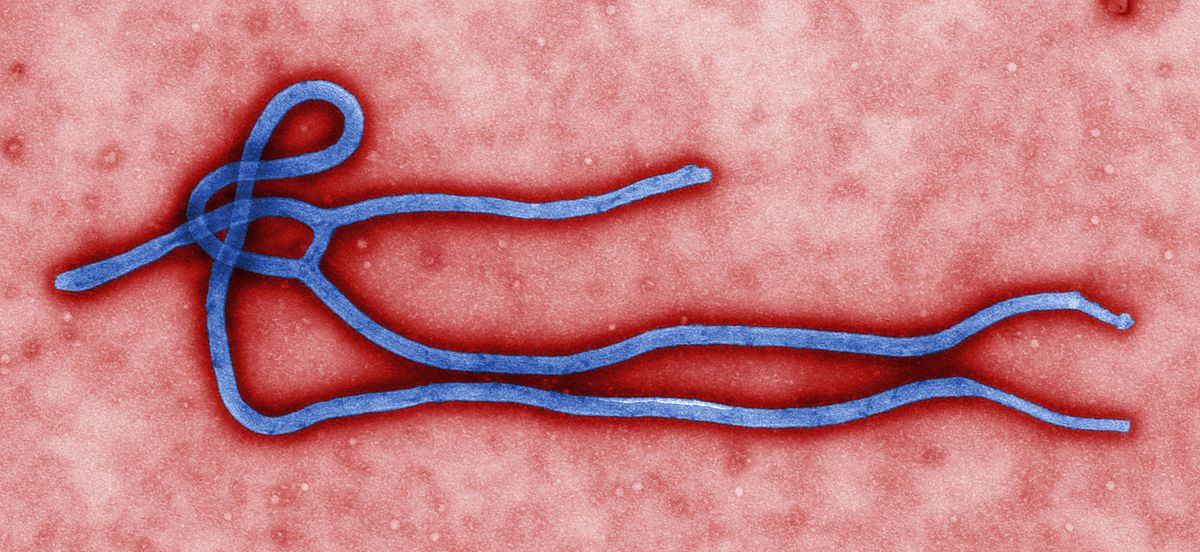
\includegraphics[scale=0.5]{ebola.jpg}
\end{center}
A patient goes to the doctor because he as a fever. Define
\begin{center}
\begin{tabular}{ll}
$H \equiv $ & ``The patient has Ebola''\\
$\neg H \equiv $ & ``The patient does not have Ebola''.
\end{tabular}
\end{center}

\end{frame}

\begin{frame}[t]{Updating Probabilities: Example}
Based on all of her knowledge, the doctor assigns probabilities to the two
hypotheses.
\begin{eqnarray*}
P(H) &=& 0.01\\
P(\neg H) &=& 0.99
\end{eqnarray*}

But she wants to test the patient to make sure.
\end{frame}



\begin{frame}[t]{Updating Probabilities: Example}
The patient is tested. Define

\begin{center}
\begin{tabular}{ll}
$D \equiv $ & ``The {\bf test says} the patient has Ebola''\\
$\neg D \equiv $ & ``The {\bf test says} the patient does not have Ebola''.
\end{tabular}
\end{center}

If the test were perfect, we'd have $P(D | H) = 1$, $P(\neg D | H) = 0$,
$P(D | \neg H) = 0$, and $P(\neg D | \neg H) = 1$.
\end{frame}


\begin{frame}[t]{Updating Probabilities: Example}
The Ebola test isn't perfect. Suppose there's a 5\% probability it simply gives
the wrong answer. Then we have:

\begin{eqnarray*}
P(D | H)   &=& 0.95\\
P(\neg D | H) &=& 0.05\\
P(D | \neg H)   &=& 0.05\\
P(\neg D | \neg H) &=& 0.95
\end{eqnarray*}

\end{frame}

\begin{frame}[t]{Updating Probabilities: Example}
Overall, there are four possibilities, considering whether the patient has
Ebola or not, and what the test says.

\begin{center}
$(H, D)$\\
$(\neg H, D)$\\
$(H, \neg D)$\\
$(\neg H, \neg D)$
\end{center}


\end{frame}

\begin{frame}[t]{Updating Probabilities: Example}
The probabilities for these four possibilities can be found using the product
rule.
\begin{eqnarray*}
P(H, D) &=& 0.01 \times 0.95\\
P(\neg H, D) &=& 0.99 \times 0.05\\
P(H, \neg D) &=& 0.01 \times 0.05\\
P(\neg H, \neg D) &=& 0.99 \times 0.95\\
\end{eqnarray*}
\vspace{-45pt}

These four possibilities are {\bf mutually exclusive} (only one of them is true)
and exhaustive (it's not ``something else''), so the probabilities add up to 1.

\end{frame}

\begin{frame}[t]{Updating Probabilities: Example}
The test results come back and say that the patient has Ebola. That is, we've
learned that $D$ is true. So we can confidently rule out those possibilities
where $D$ is false:

\begin{eqnarray*}
P(H, D) &=& 0.01 \times 0.95\\
P(\neg H, D) &=& 0.99 \times 0.05\\
{\color{red} P(H, \neg D)} &=& {\color{red} 0.01 \times 0.05}\\
{\color{red} P(\neg H, \neg D)} &=& {\color{red} 0.99 \times 0.95}\\
\end{eqnarray*}


\end{frame}


\begin{frame}[t]{Updating Probabilities: Example}
We are left with these two possibilities.

\begin{eqnarray*}
P(H, D) &=& 0.01 \times 0.95\\
P(\neg H, D) &=& 0.99 \times 0.05
\end{eqnarray*}

It would be strange to modify these probabilities just because we deleted the
other two. The only thing we have to do is renormalise them, by dividing by the total, so they sum to 1 again.
\end{frame}

\begin{frame}[t]{Updating Probabilities: Example}
Normalising, we get

\begin{eqnarray*}
P(H | D) &=& (0.01 \times 0.95)/(0.01 \times 0.95 + 0.99\times0.05) = 0.161\\
P(\neg H | D) &=& (0.99 \times 0.05)/(0.01 \times 0.95 + 0.99\times0.05) = 0.839
\end{eqnarray*}
\end{frame}

\begin{frame}[t]{Moral}
Bayesian updating is completely equivalent to:
\begin{itemize}
\item Writing a list of possible answers to your question
\item Giving a probability to each
\item Deleting the ones that you discover are false.
\end{itemize}

It just seems more complicated than this because we often apply it to more
complex sets of hypotheses.
\end{frame}


% New slide
\begin{frame}
\frametitle{Basic Bayesian exercises}

Do exercise set 1.

\end{frame}



\end{document}


